

\section{Pan e Tilt}
\label{encoder}


\begin{table}[ht!]

	\begin{tabular}{r l|l p{12cm} }
		
		\textcolor{gray}{Especificação} &&& 	{Pan e Tilt - OE10-102}\\
		\textcolor{gray}{Data} &&& 				{??/2014}\\
        \textcolor{gray}{Beneficiado} &&&		{Kongsberg} \\
        \textcolor{gray}{CNPJ} &&& 				{Internacional} \\
        \textcolor{gray}{Número Nota} &&& 		{Pendente - Produto em trânsito} \\
		\textcolor{gray}{Quantidade} &&& 		{1} \\
		\textcolor{gray}{Valor} &&& 			{R\$39.358,18} \\
		\textcolor{gray}{Data Sheet} &&& 		{Anexo IV - \ref{datasheet_pantilt} } \\

		\textcolor{gray}{Função no projeto} &&& {O motor de posicionamento será acoplado ao Sonar 2D aumento o grau de liberdade do sistema de mapeamento, possibilitando assim cobrir toda a extensão do trilho do Stoplog.} \\
		\textcolor{gray}{Razão da Escolha} &&& {O fator mais importante na escolha do motor de posicionamento é a precisão que o mesmo consegue operar, pois o sonar mede a distância ao meio que se encontra de 3 a 50 metros de distância do mesmo, logo um pequeno erro de posicionamento angular do motor resultará em um erro grande na reconstrução do meio. Exemplo: 1 grau de erro a 50m de distância significaria 0,87m de erro na reconstrução do ambiente. Logo, o modelo escolhido para o projeto foi o OE10-102 que oferece a menor folga mecânica. 
		\begin{itemize}
		  \item \textbf{OE10-102 da Kongsber com 0.08 graus por \$12.563} 
		  \item SS109 da Sidus com 0.5 graus por \$6.220 dolares, data sheet em anexo \ref{datasheet_pantilt} 
		  \item PT-10FB da ROS com 0.6 graus por \$10.285, data sheet em anexo \ref{datasheet_pantilt} 
		\end{itemize}}
		

	\end{tabular}
\end{table}



\begin{figure}[h!]
 \centering
 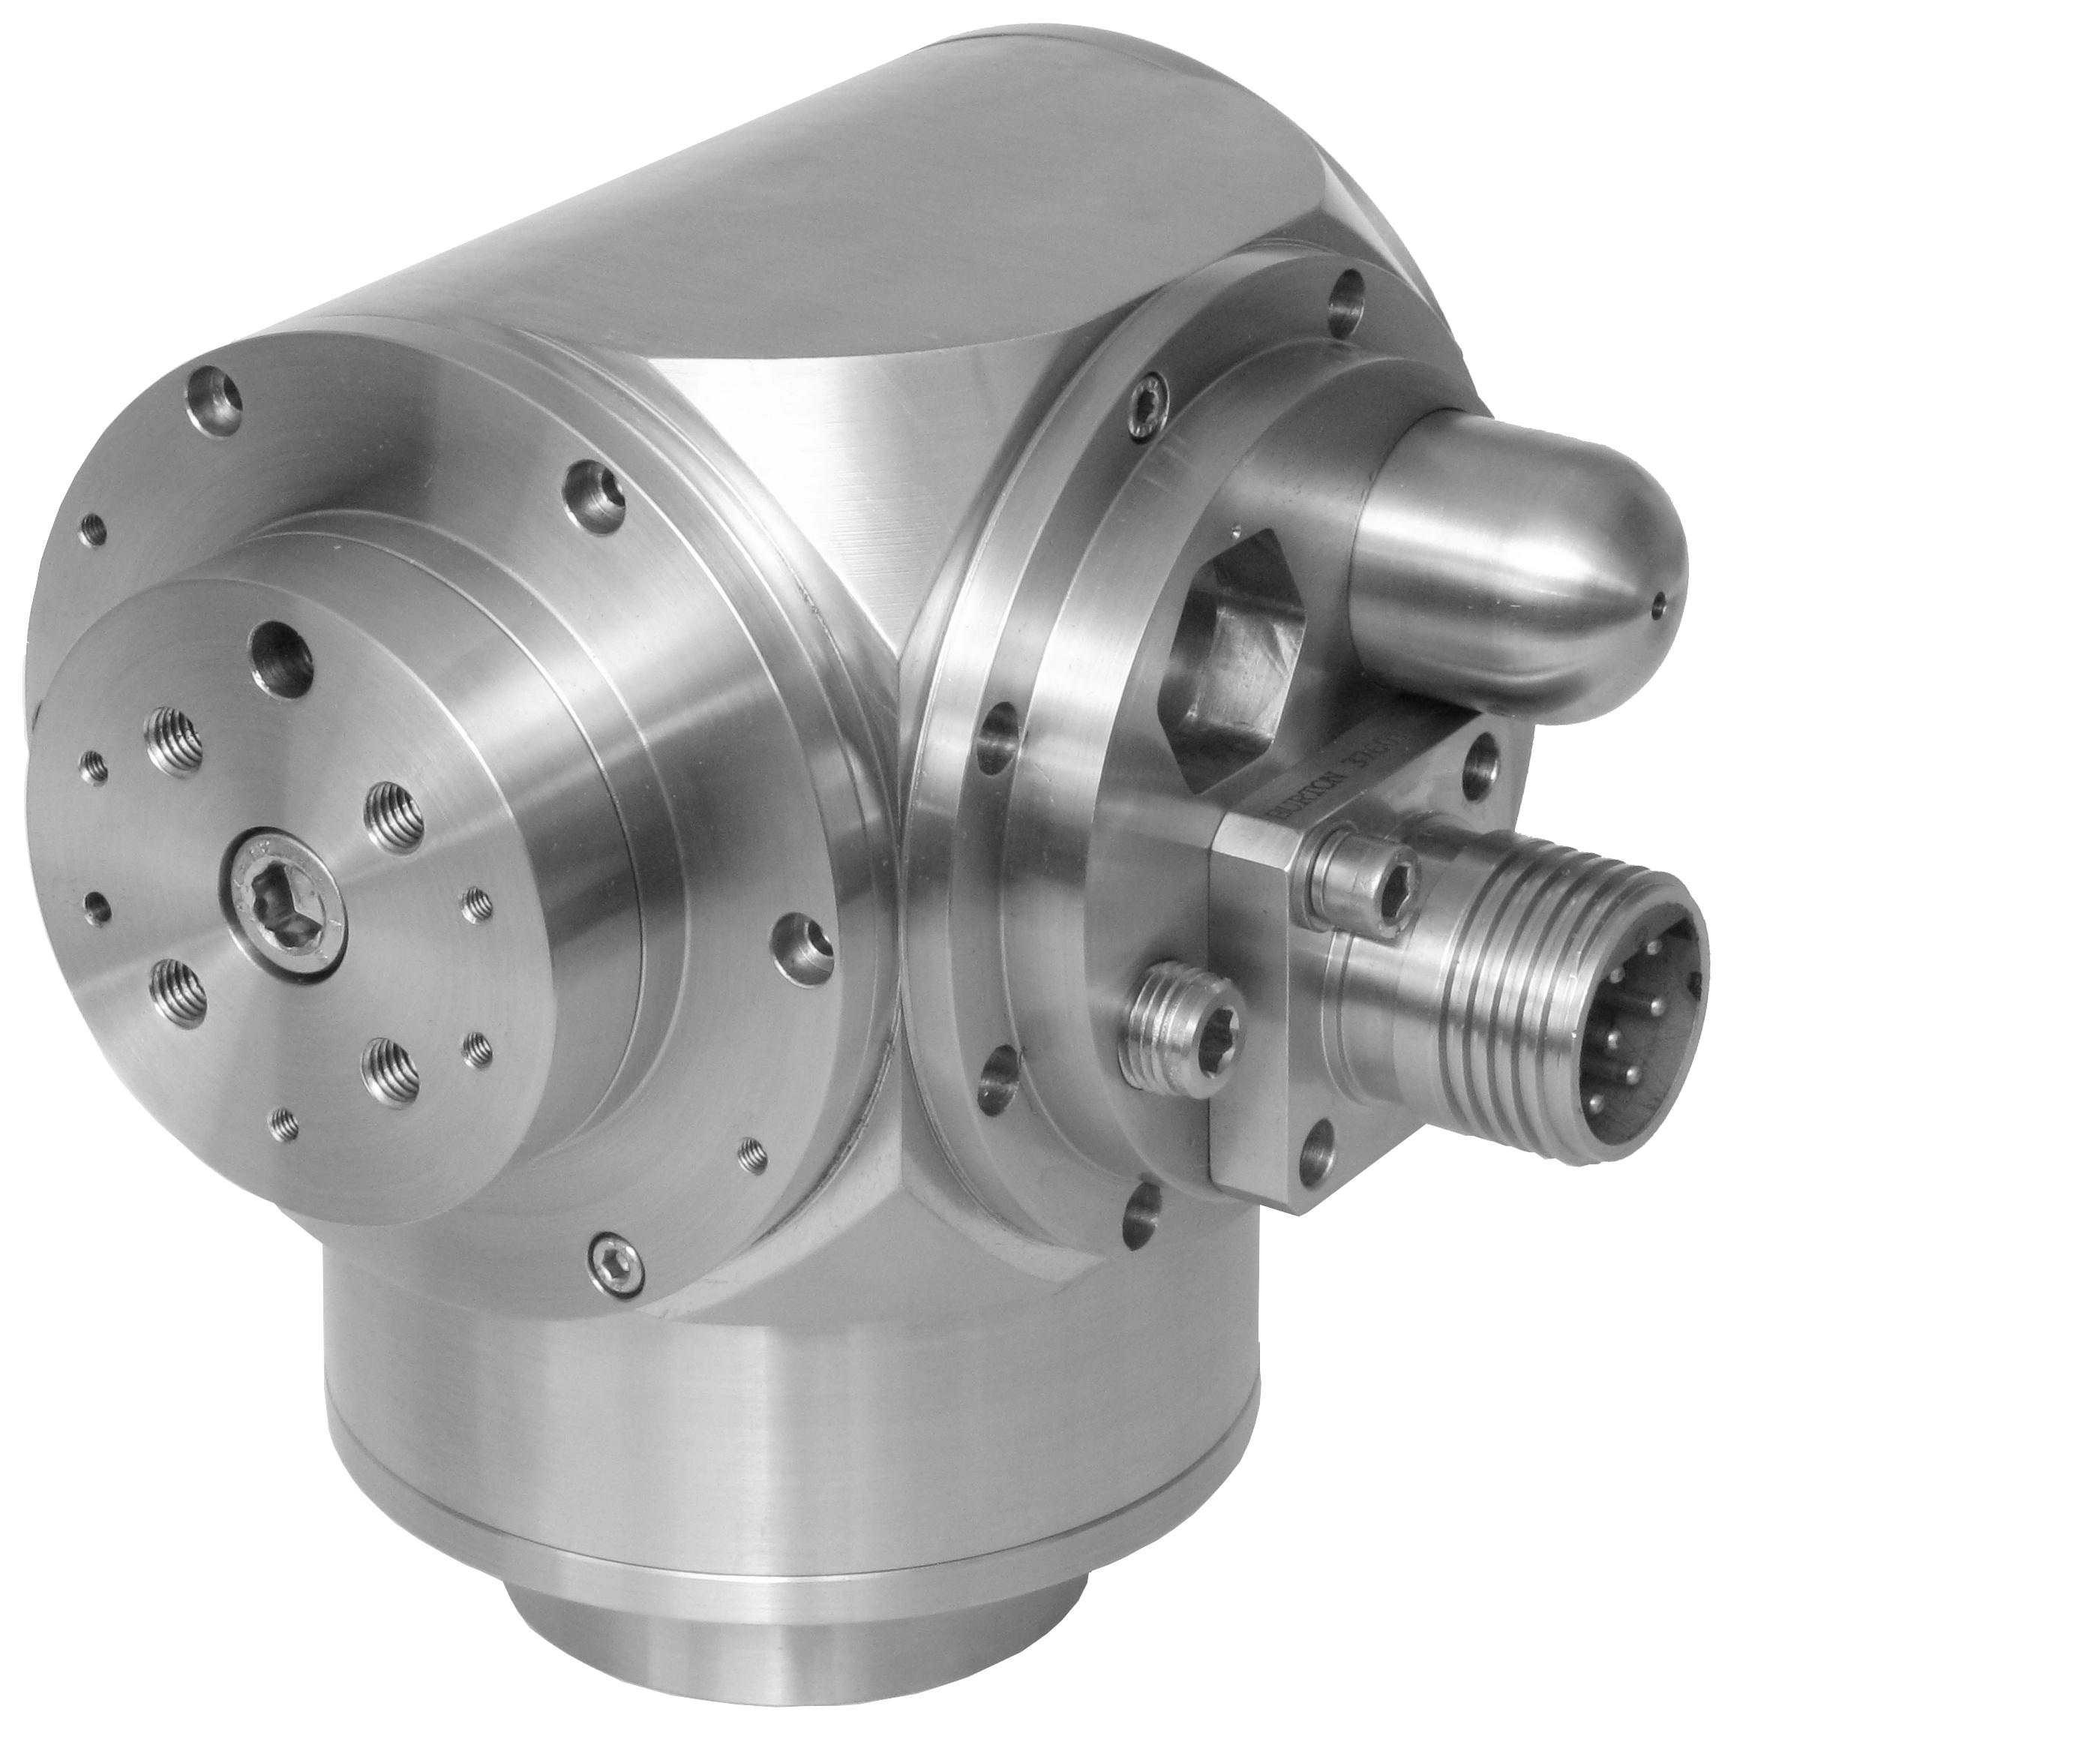
\includegraphics[width=0.3\columnwidth]{Pan_Tilt/foto}
 \caption{OE10-102 da Kongsber}
  
\end{figure}



\begin{figure}[h!]
\centering
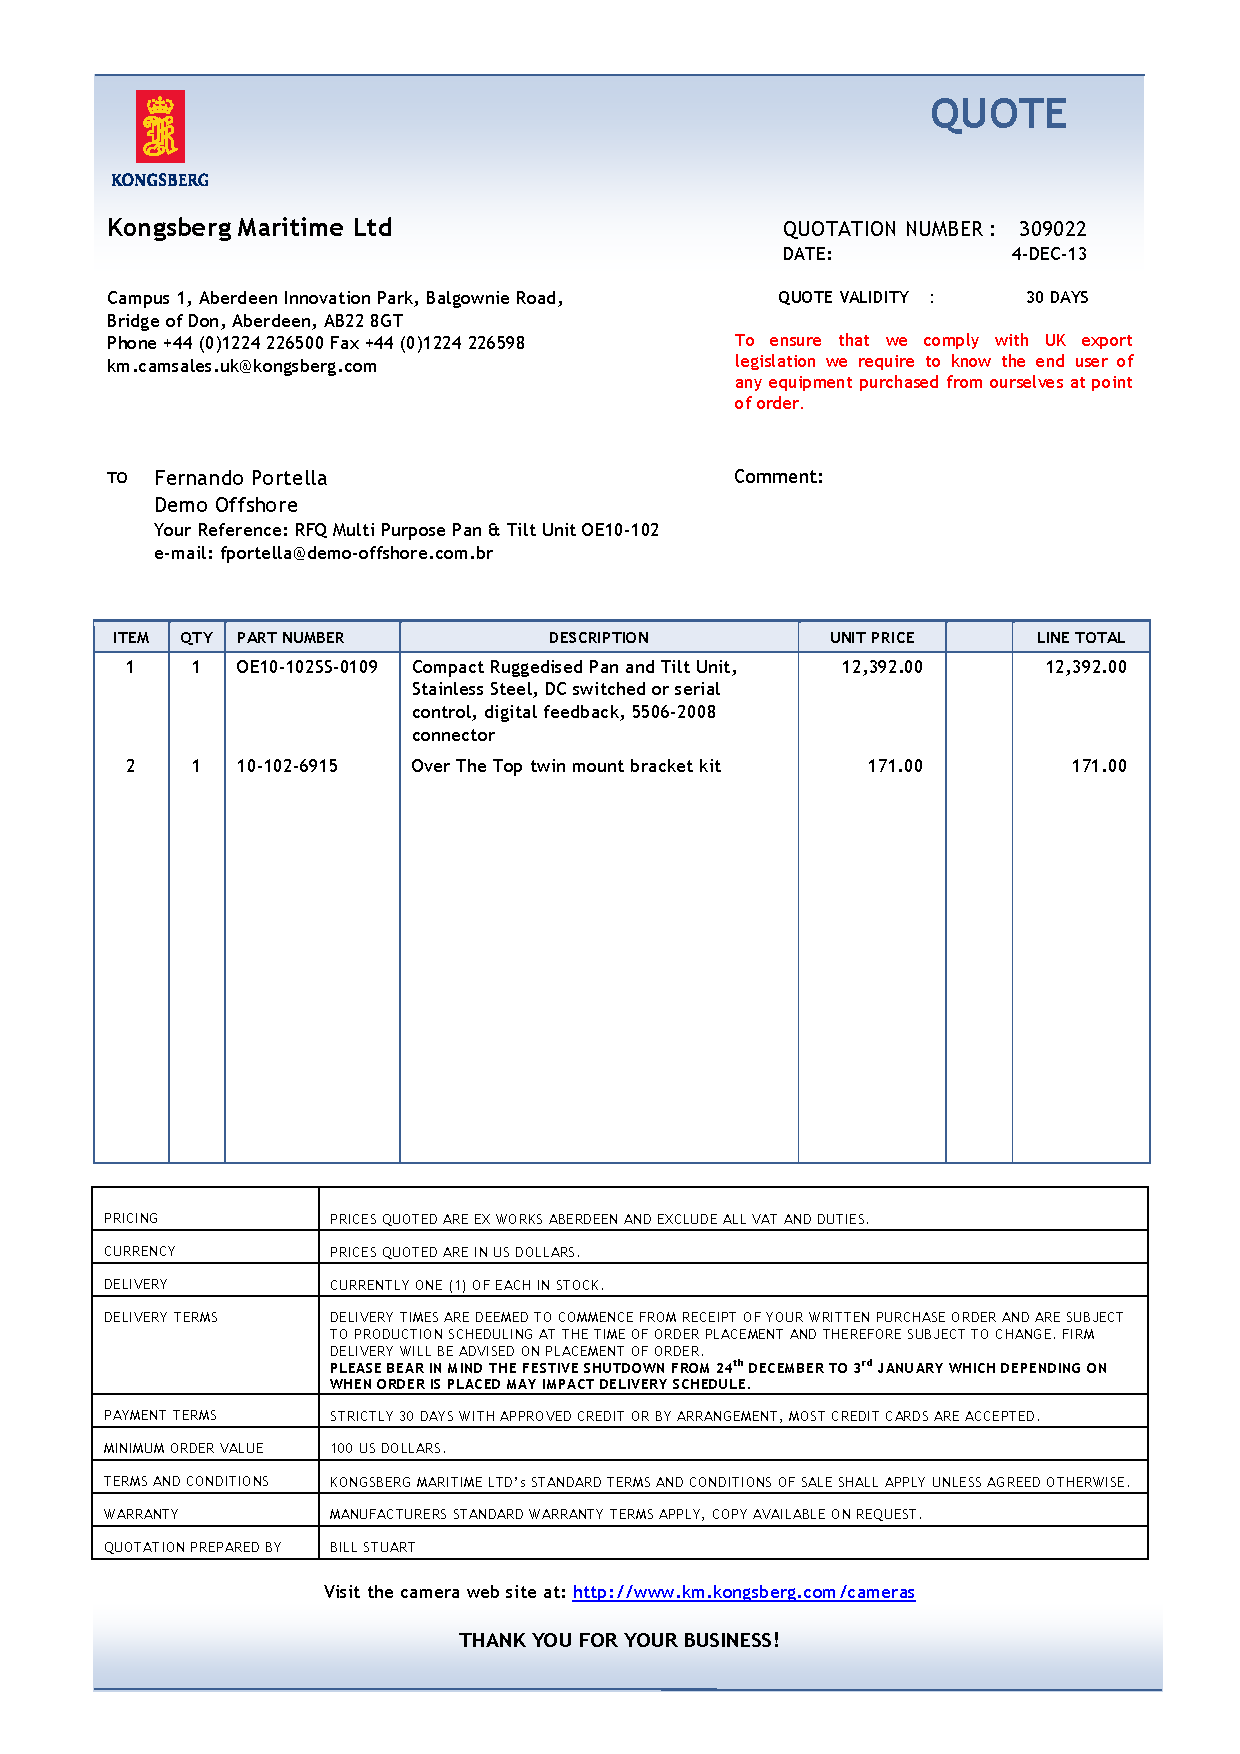
\includegraphics[width=1\columnwidth]{Pan_Tilt/price_quote_0.pdf}
\caption{Cotação OE10-102 da Kongsber  } 
\end{figure}

\begin{figure}[h!]
 \centering
 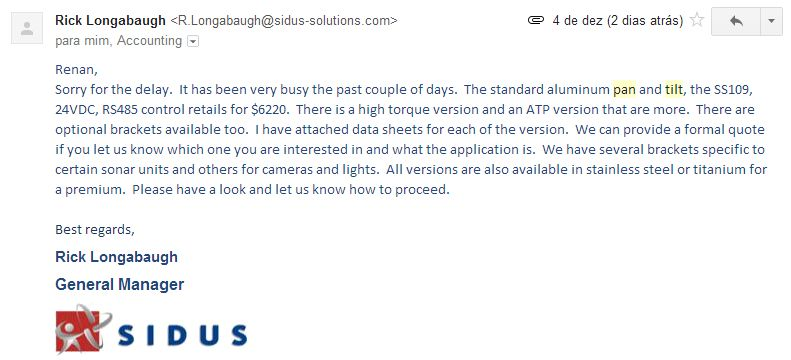
\includegraphics[width=1\columnwidth]{Pan_Tilt/price_quote_1}
 \caption{Cotação SS109 da Sidus}
\end{figure}

\begin{figure}[h!]
 \centering
 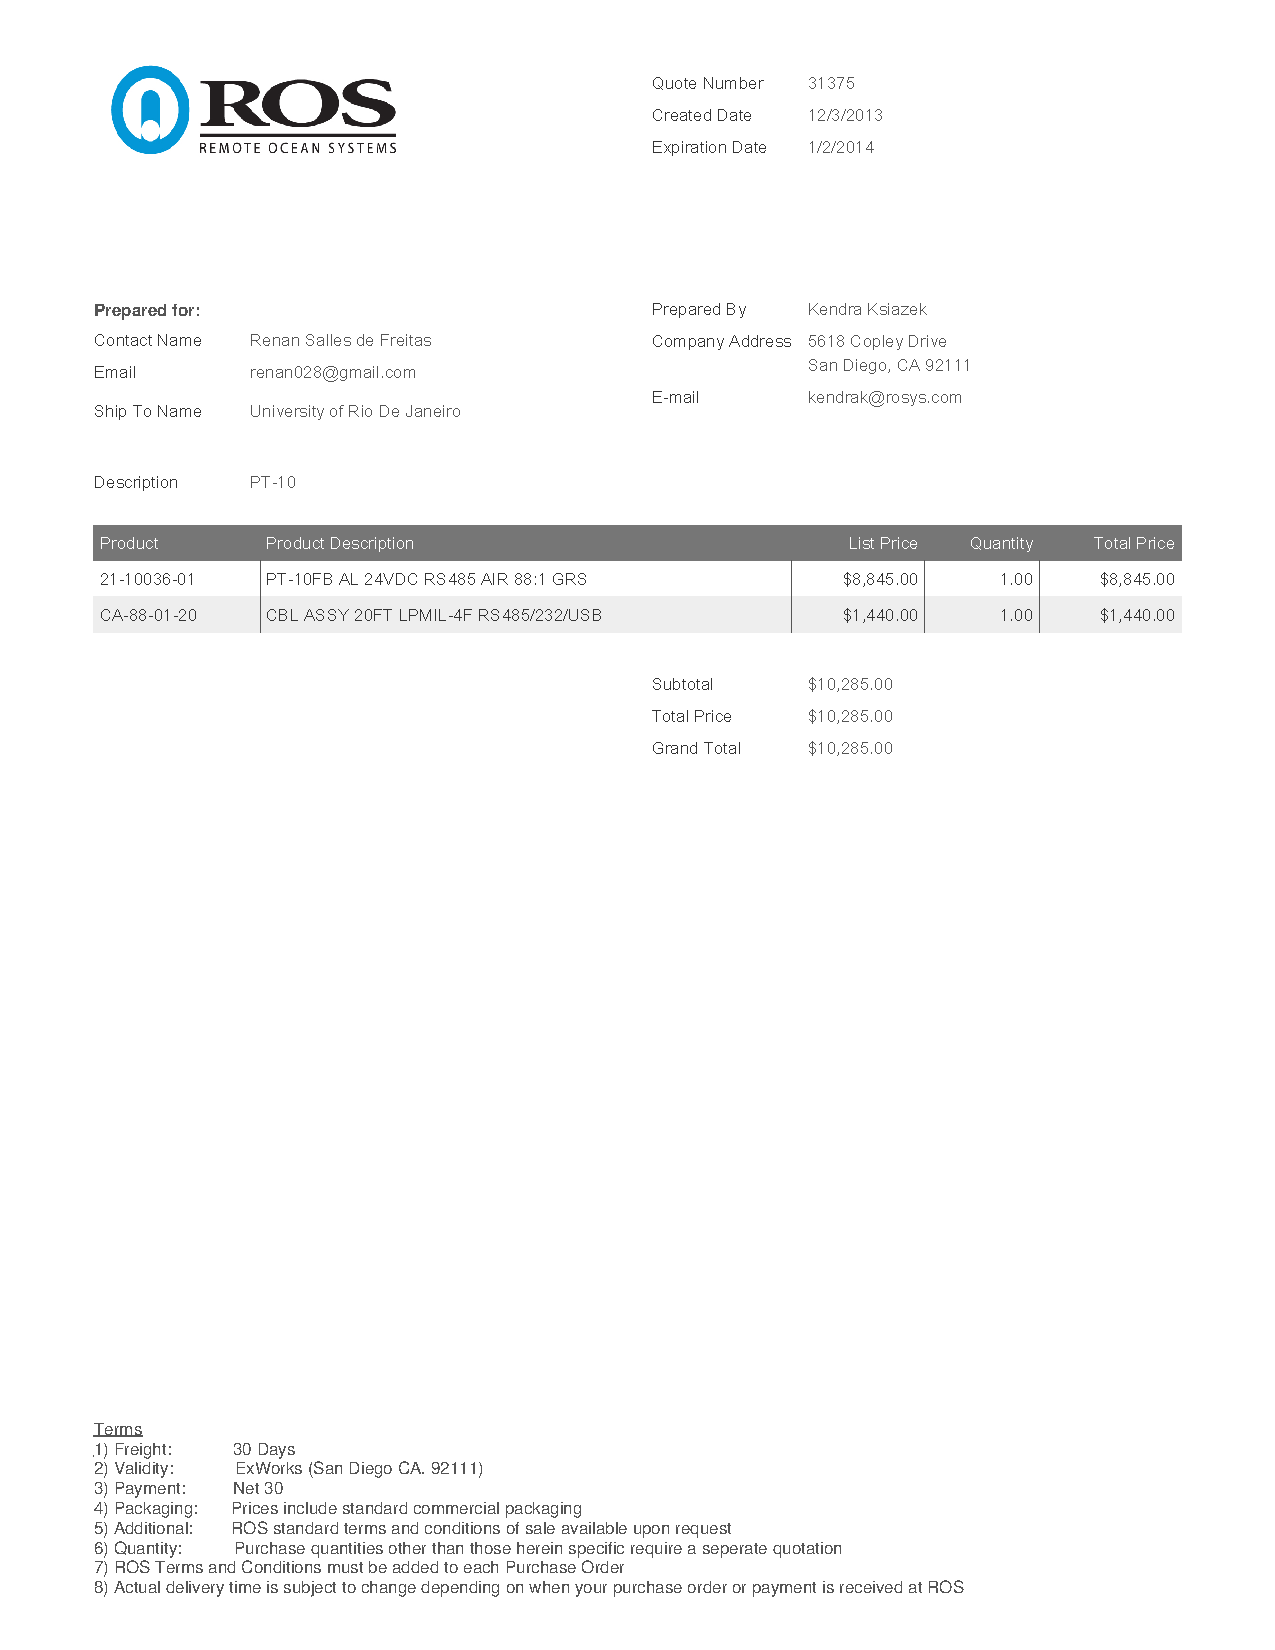
\includegraphics[width=1\columnwidth]{Pan_Tilt/price_quote_2}
 \caption{Cotação PT-10FB da ROS } 
\end{figure}